\documentclass[spanish]{article}
\usepackage{graphicx}
\usepackage{ragged2e}
\usepackage{geometry}
\usepackage{float}
\usepackage{hyperref}
\usepackage[table,xcdraw]{xcolor}
\usepackage[ruled,vlined]{algorithm2e}
\title {Práctica 5: Algoritmos Greedy}
\graphicspath{{../img/}}
\addtolength{\textheight}{1.5in} 
\begin{document}
	\centerline{
\includegraphics[width=450px,height=100px]{header}}
	\centerline{Analisis de algoritmos, Sem: 2021-1, 3CV1,Práctica  3, 11/11/2020}
	\centering{\huge{Práctica 5: Algoritmos Greedy}}
	\centerline{\newline{\textbf{Payán Téllez René}}}
	\newline{\textit{rpayant1500@alumno.ipn.mx}}
	\bigskip
	\justify
	\textbf{Resumen:}	
	En esta practica se analizaran 2 algoritmos que utilizan la tecnica de divide y venceras para resolver un problema, uno de ellos el quick sort y otro el sub arreglo maximo.\\
	\textbf{Palabras clave:}
	QuickSort,SubArreglo maximo,divide y venceras,C/C++
	\section{Introduccion}
	
	\section{Conceptos Basicos}
	\subsection{Algoritmo}
		La palabra algoritmo proviene del sobrenombre de un matemático árabe del siglo IX, Al-Khwarizmi, que fue reconocido por enunciar paso a paso las reglas para las operaciones matemáticas básicas con decimales (suma, resta, multiplicación y división).	
		Vemos definición de algoritmo como un grupo de órdenes consecutivas que presentan una solución a un problema o tarea. Algunos ejemplos de algoritmos los podemos encontrar en las matemáticas (como el algoritmo para resolver una multiplicación) y en los manuales de usuario de un aparato (como una lavadora o una impresora).	
		Sin embargo, hoy en día se relaciona la palabra algoritmo con el mundo de la informática, más concretamente en la programación; los conocidos como algoritmos informáticos.[1]
	\subsection{Complejidad algoritmica}
		Así que, por su naturaleza, un problema tiene la capacidad de ser solucionado por uno o varios métodos, pero si bien es importante llegar a la respuesta, más importante es evaluar su viabilidad. Siempre que se analiza y evalúa adecuadamente la efectividad de una solución, disminuye drásticamente el costo que representa su producción y mantenimiento, pues los recursos que se invierten posteriormente en codificación, pruebas y revisión es mucho menor siempre (como el tiempo, dinero y talento humano).	
		Entrando en materia, la complejidad algorítmica es una métrica teórica que nos ayuda a describir el comportamiento de un algoritmo en términos de tiempo de ejecución (tiempo que tarda un algoritmo en resolver un problema) y memoria requerida (cantidad de memoria necesaria para procesar las instrucciones que solucionan dicho problema). Esto nos ayuda a comparar entre la efectividad de un algoritmo y otro, y decidir cuál es el que nos conviene implementar.[2]
	\subsection{Algoritmos Greedy o glotones}	
		Un algoritmo Greedy o gloton es un algoritmo muy util para encontrar soluciones aproximadas e inclusive la mas optima a problemas complejos, ya que las entregan en muy corto tiempo. Se llaman Greedy porque siempre "comen lo que tienen a la mano", no garantizan encontrar la mejor solucion, pero si una aproximacion bastante buena.[3]
		Estas son sus caracteristicas principales:
		\begin{itemize}
			\item Se utilizan generalmente para resolver problemas deoptimización (obtener el máximo o el mínimo).optimización (obtener el máximo o el mínimo).
			\item Toman decisiones en función de la información que está disponible en cada momento. está disponible en cada momento. está disponible en cada momento. está disponible en cada momen
			\item Una vez tomada la decisión, ésta no vuelve a replantearse en el futuro.replantearse en el futuro.
			\item Suelen ser rápidos y fáciles de implementar.
			\item No siempre garantizan alcanzar la solución óptima[4]
		\end{itemize}
	\subsection{Algoritmo de codificación de Huffman}
		El código de Huffman es un tipo particular de código de prefijo óptimo que se usa comúnmente para la compresión de datos sin pérdida. Comprime los datos de manera muy efectiva, ahorrando de 20$\%$ a 90$\%$ de memoria, dependiendo de las características de los datos comprimidos. Este algoritmo se aplica solo si se considera a la entrada como una cadena de caracteres, ya que es un algoritmo boraz que utiliza una tabla que proporciona la frecuencia con la que aparece cada carácter (es decir, su frecuencia) para crear una forma óptima de representar cada carácter como una cadena binaria. Fue propuesto por David A. Huffman en 1951.[5]
		\begin{algorithm}[H]
			\KwData{Entrada: C (Los caracteres de la cadena a codificar y su ocurrencia)}
			\KwResult{Retorna el arbol de huffman de la cadena}
			n = C.size\;
			Q = priority\_queue();
			\For{$i\gets 0$ \KwTo $i < n$}{
				n=node(C[i])
				Q.push(n)
			}
			\While{Q.size()>1}{
				Z = new node()\;
				Z.left = x = Q.pop()\;
				Z.right = y = Q.pop()\;
				Z.frequency = x.frequency+y.frequency\;
				Q.push(Z)\;
				
			}
			return Q\;
			\caption{HuffmanTree(C)}
		\end{algorithm}
		\begin{algorithm}[H]
			\KwData{Entrada: tree (El arbol de Huffman), S (la cadena binaria a descomprimir)}
			\KwResult{Retorna una cadena de caracteres descomprimida}
			n = S.length\;
			retorno = ""\;
			\For{$i\gets 0$ \KwTo $i < n$}{
				current = root\;
				\While{current.left != NULL and current.right!=NULL}{
					\If{S[i] == '0'}{
						current = current.left\;					
					}
					\Else{
						current = current.right\;											
					}
				}
				i+=1\;
				retorno+=current.symbol\;
			}
			return retorno\;
			\caption{HuffmanDecompression(tree, S)}
		\end{algorithm}
		\subsection{Algoritmos de Kruskal}
	\begin{algorithm}[H]
		\KwData{Entrada: A[0,...,n-1], bajo, mitad, alto}
		\KwResult{Retorna la suma del mayor sub arreglo de la izquierda, la derecha y juntos}
		suma\textunderscore izq=INT\textunderscore  MIN\;
		suma=0\;
		max{\textunderscore}izq=0\;
		\For{$i\gets mitad\   \KwTo\   bajo$}{
			suma+=A[i]\;
			\If{$suma>suma\_izq$}{
				suma{\textunderscore}izq=suma\;
				max{\textunderscore}izq=i\;	
			}
		}
		suma{\textunderscore}der=INT{\textunderscore}MIN\;
		suma=0\;
		max{\textunderscore}der=0\;
		\For{$j\gets mitad\   \KwTo\   alto$}{
			suma+=A[j]\;
			\If{$suma>suma\_der$}{
				suma{\textunderscore}der=suma\;
				max{\textunderscore}der=j\;			
			}
		}
		return (max{\textunderscore}izq,max{\textunderscore}der,suma{\textunderscore}der+suma{\textunderscore}izq)\;
		\caption{MaxCrossingSubArray(A[0,...,n-1],bajo,mitad,alto)}		
	\end{algorithm}
	\begin{algorithm}[H]
		\KwData{Entrada: A[0,...,n-1], bajo, alto}
		\KwResult{retorna la suma y los indices del mayor sub arreglo, que se puede obtener dentro del arreglo A}
		\If{alto == bajo}{
			return(bajo,alto,A[bajo])\;
		}
		\Else{
			mitad=$\frac{bajo+alto}{2}$\;
			(bajo$\_$izq,alto$\_$izq,suma$\_$izq)=MaxSubArrayDC(A,bajo,mitad)\;
			(bajo$\_$der,alto$\_$der,suma$\_$der)=MaxSubArrayDC(A,mitad+1,alto)\;
			(cruz$\_$izq,cruz$\_$der,suma$\_$cruz)=MaxCrossingSubArray(A,bajo,mitad,alto)\;
			\If{$suma\_izq>suma\_der$\ and $suma\_izq>suma\_cruz$}{
				return (bajo$\_$izq,alto$\_$izq,suma$\_$izq)\;				
			}\ElseIf{$suma\_der>suma\_izq$\ and $suma\_der>suma\_cruz$}{
				return (bajo$\_$der,alto$\_$der,suma$\_$der)\;				
			}\Else{
				return (cruz$\_$izq,cruz$\_$der,suma$\_$cruz)\;
			}
		}		
		return (max{\textunderscore}izq,max{\textunderscore}der,suma{\textunderscore}der+suma{\textunderscore}izq)\;
		\caption{MaxSubArrayDC(A[0,...,n-1],bajo,alto)}
	\end{algorithm}
	\newpage
	\begin{algorithm}[H]
		\KwData{Entrada: A[0,...,n-1]}
		\KwResult{Retorna la suma y los indices del mayor sub arreglo, que se puede obtener dentro del arreglo A}
		sumaMaxima=$-\infty$\;
		indiceIzquierdo = 0\;
		indiceDerecho = 0\;
		\For{$i\gets 0\   \KwTo\   n$}{
			sumaLocal=0\;
			\For{$j\gets i\   \KwTo\   n$}{
				sumaLocal+=A[j]\;
				\If{sumaLocal$>$sumaMaxima}{
					sumaMaxima = sumaLocal\;
					indiceIzquierdo=i\;
					indiceDerecho=j\;
				}			
			}
		}
		return(sumaMaxima,indiceIzquierdo,indiceDerecho)\;
		\caption{FuerzaBruta(A[0,...,n-1])}
	\end{algorithm}
	\section{Experimentacion y Resultados}
	\subsection{Implementar el algoritmo de codificacion de Huffman.}
	Para esta primera parte de pruebas se implemento el algoritmo de codificacion y decodificacion de Huffman, asi que la ejecución se divide en 2 partes, la compresion de una cadena de texto y para la segunda parte la descompresion de la misma
	\begin{figure}[H]
		\centering
		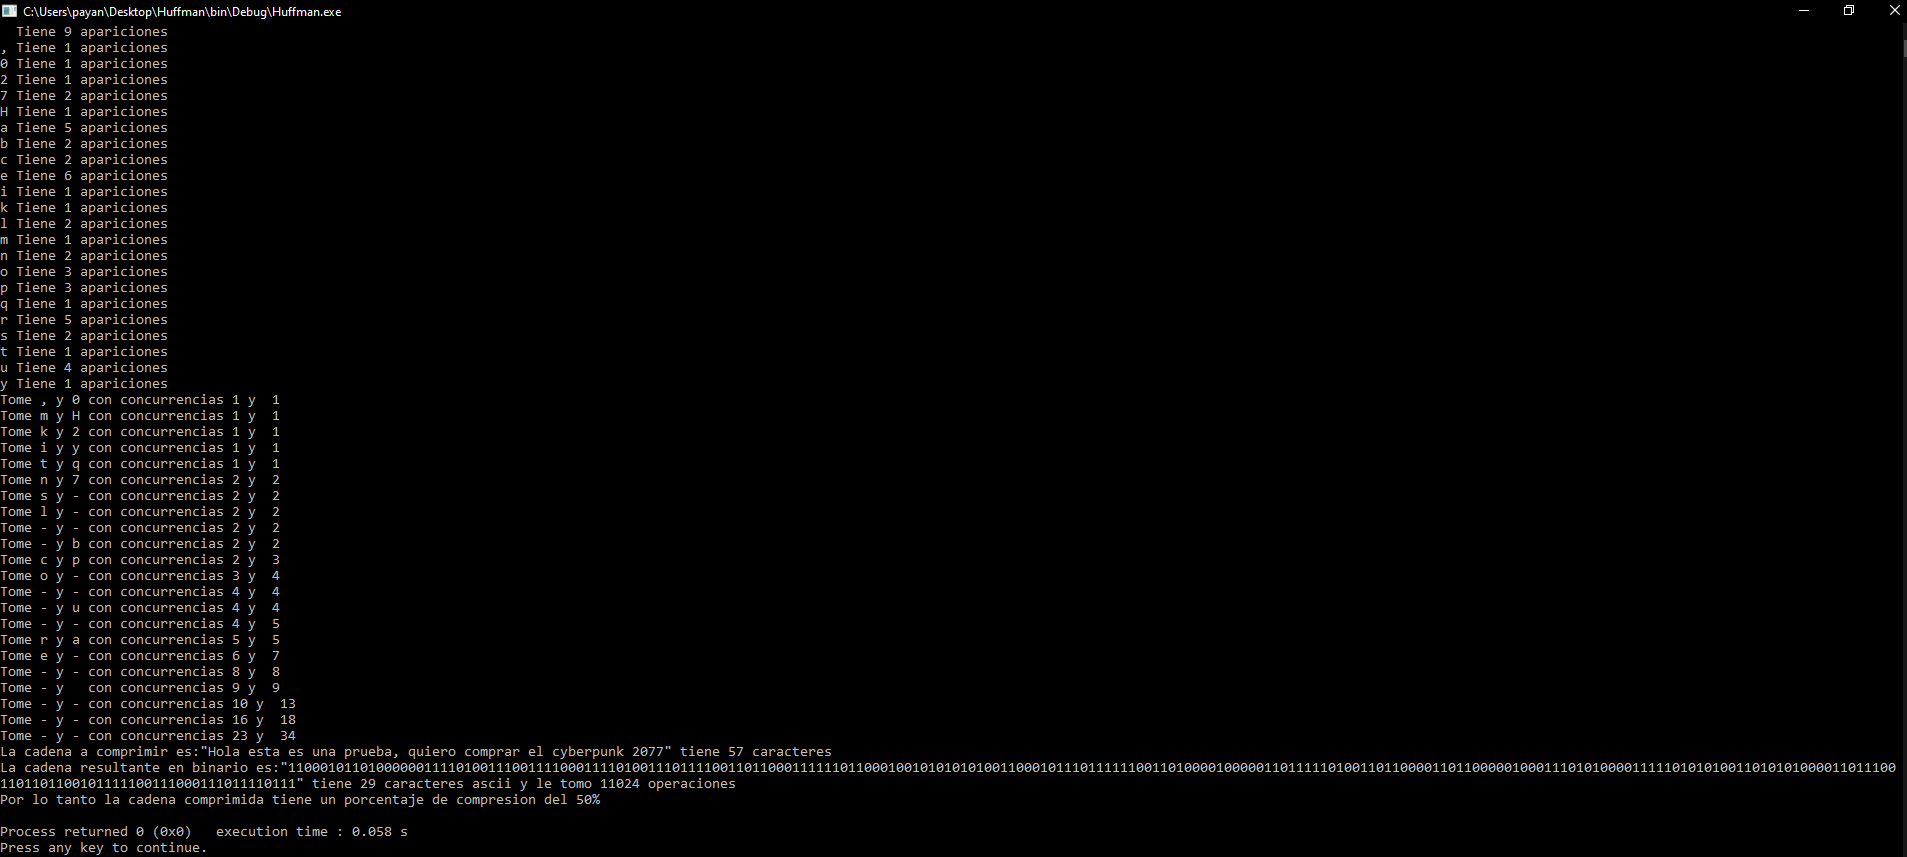
\includegraphics[width=400px,height=300px]{captura1}
		\caption{Compresión de la cadena "Hola esta es una prueba, quiero comprar el cyberpunk 2077"}
	\end{figure}
	
	\begin{figure}[H]
		\centering
		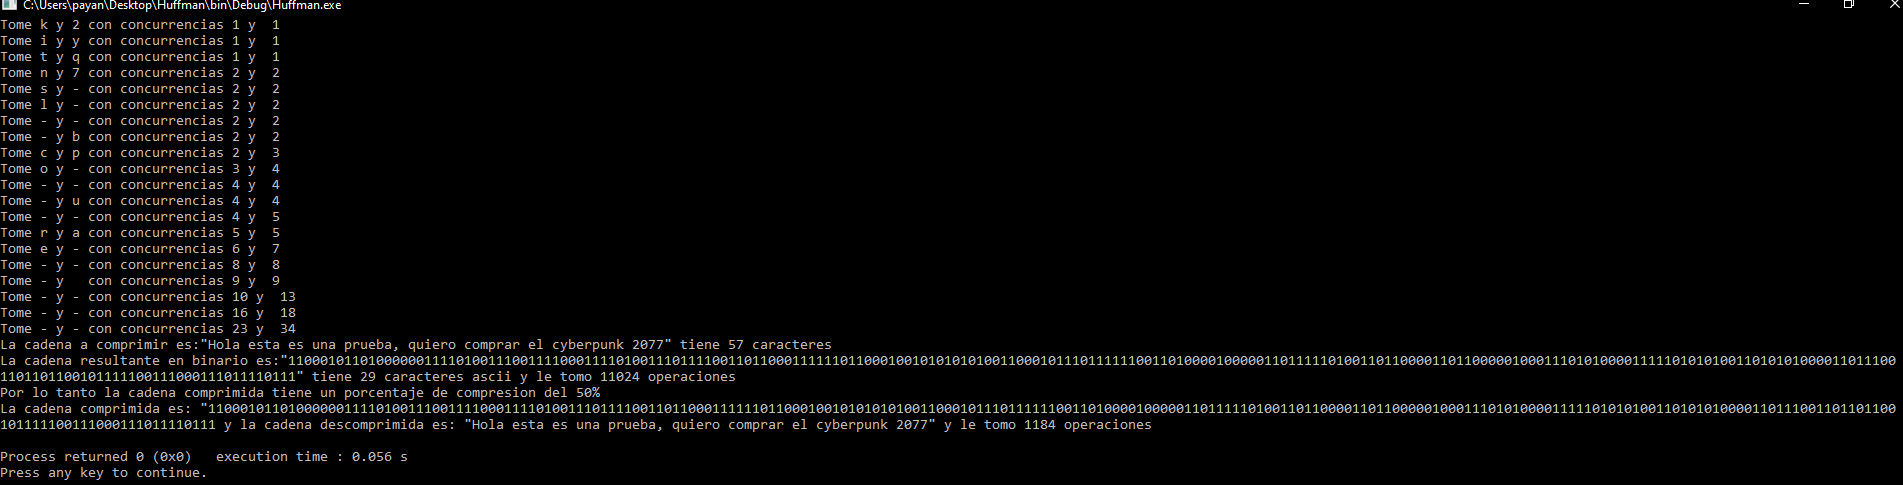
\includegraphics[width=400px,height=300px]{captura2}
		\caption{Descompresión  de la cadena "Hola esta es una prueba, quiero comprar el cyberpunk 2077"}
	\end{figure}
	Como se pudo apreciar en las capturas, la capturas, el programa tomo la entrada "Hola esta es una prueba, quiero comprar el cyberpunk 2077" y retorno la siguiente salida como respuesta: "", posteriormente al introducir la salida de la compresion en la seccion de descompresion, el programa arrojo la cadena original.
	Podemos decir que el algoritmo es eficiente, porque esta es la cantidad de caracteres de la cadena original:
	\begin{figure}[H]
		\centering
		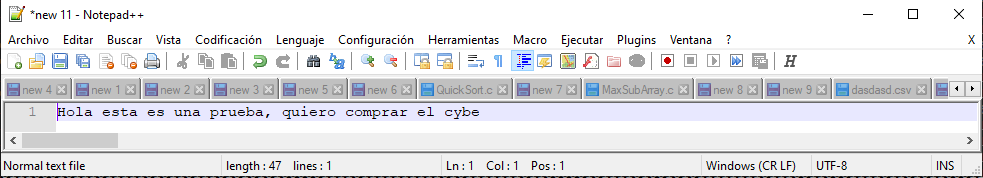
\includegraphics[width=400px,height=150px]{captura3}
		\caption{Conteo de caracteres de la entrada}
	\end{figure}
	esta es la cantidad de caracteres de la salida:
	\begin{figure}[H]
		\centering
		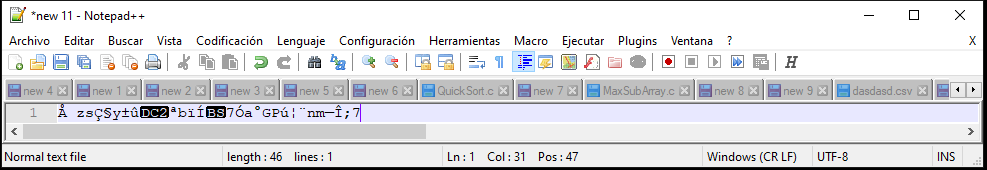
\includegraphics[width=400px,height=150px]{captura4}
		\caption{Conteo de caracteres de la salida}
	\end{figure}
	por ultimo, el binario de cada caracter asignado
	\begin{figure}[H]
		\centering
		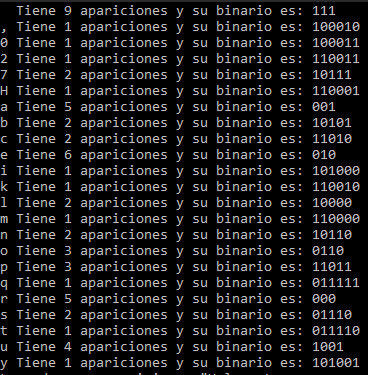
\includegraphics[width=400px,height=300px]{captura9}
		\caption{Asignacion de binario}
	\end{figure}
	A continuacion se probo con una cadena mas larga, un "Lorem Ipsum" de 1000 bytes:
	Lorem ipsum dolor sit amet, consectetur adipiscing elit. Integer porttitor turpis eget erat auctor varius. Vestibulum maximus scelerisque dui ac vulputate. Mauris eleifend mauris vel ex sodales, ut blandit odio dictum. Ut efficitur eu lectus nec ullamcorper. Integer hendrerit justo in augue consectetur, eget porttitor quam rutrum. Cras porta justo at fermentum condimentum. Nunc lacinia convallis tortor in tempor. Donec tincidunt tempor ipsum, sit amet aliquet justo semper at. Donec nibh urna, faucibus ac mauris eu, mattis imperdiet dolor. Nam et nulla at nisi efficitur efficitur. Morbi bibendum scelerisque risus, at sollicitudin ligula rutrum et. Cras sagittis eget velit aliquam cursus.
	Nunc magna metus, ullamcorper sed ante id, tincidunt ornare libero. Proin pharetra orci felis, eget pellentesque nisi venenatis eget. Morbi tincidunt ut risus non iaculis. Proin id consectetur metus, sed placerat eros. Aenean cursus augue a ipsum tempor interdum. Vivamus viverra efficitur felis a aenean. 
	\begin{figure}[H]
		\centering
		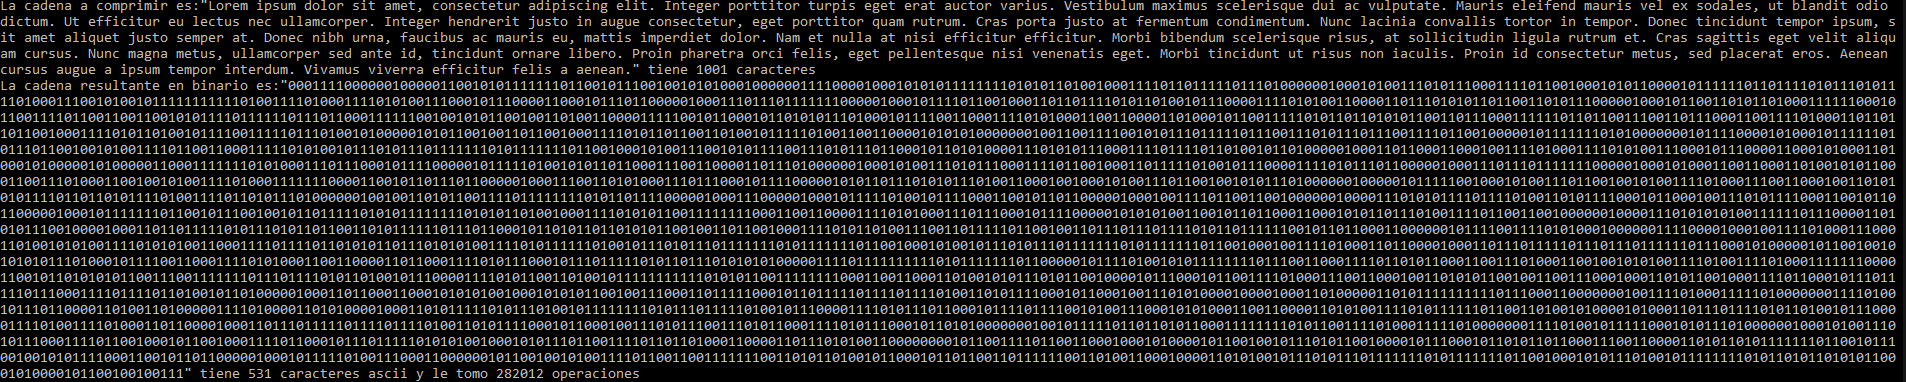
\includegraphics[width=400px,height=300px]{captura5}
		\caption{Compresión del lorem ipsum}
	\end{figure}
	
	\begin{figure}[H]
		\centering
		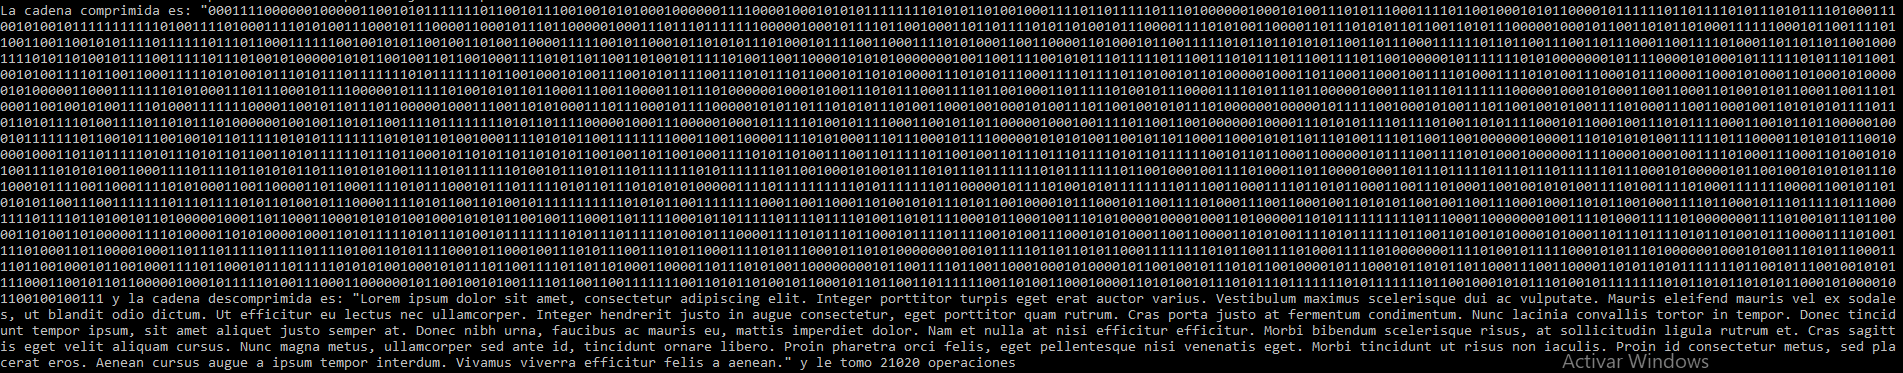
\includegraphics[width=400px,height=300px]{captura6}
		\caption{Descompresión del lorem ipsum}
	\end{figure}
	Finalmente se contaron los caractres de la entrada y de la salida:
	\begin{figure}[H]
		\centering
		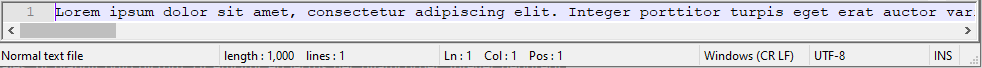
\includegraphics[width=400px,height=150px]{captura7}
		\caption{Conteo de caracteres de la entrada}
	\end{figure}
	y esta es la cantidad de caracteres de la salida:
	\begin{figure}[H]
		\centering
		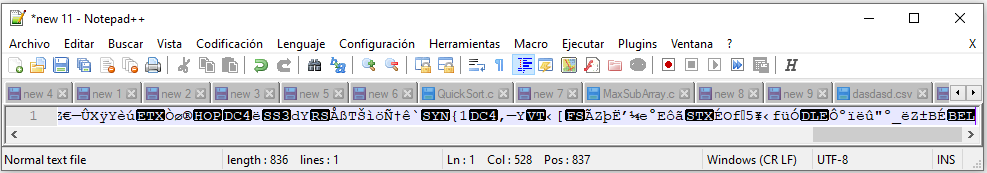
\includegraphics[width=400px,height=150px]{captura8}
		\caption{Conteo de caracteres de la salida}
	\end{figure}
	por ultimo, el binario de cada caracter asignado
	\begin{figure}[H]
		\centering
		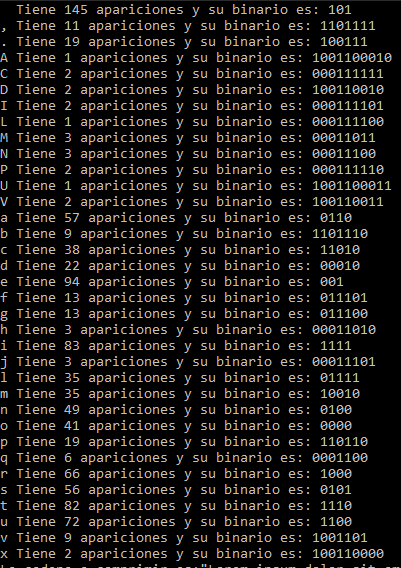
\includegraphics[width=400px,height=300px]{captura10}
		\caption{Asignacion de binario}
	\end{figure}
	A continuación se comprimieron 10 archivos de texto con extencion .txt de distinto tamaño, se anexan las capturas del binario de cada caracter, del archivo de entrada, el archivo comprimido, el archivo descomprimido y el tamaño de ambos archivos.\\
	\textbf{Primer archivo}
	\begin{figure}[H]
		\centering
		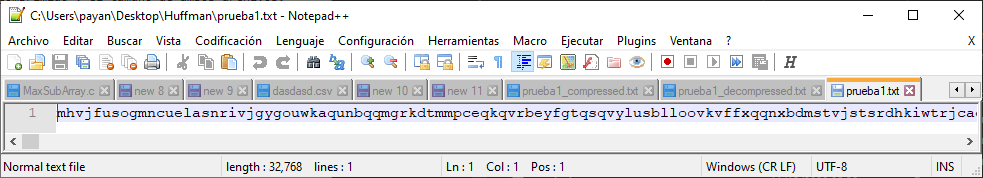
\includegraphics[width=400px,height=150px]{captura11}
		\caption{Archivo de entrada}
	\end{figure}
	\begin{figure}[H]
		\centering
		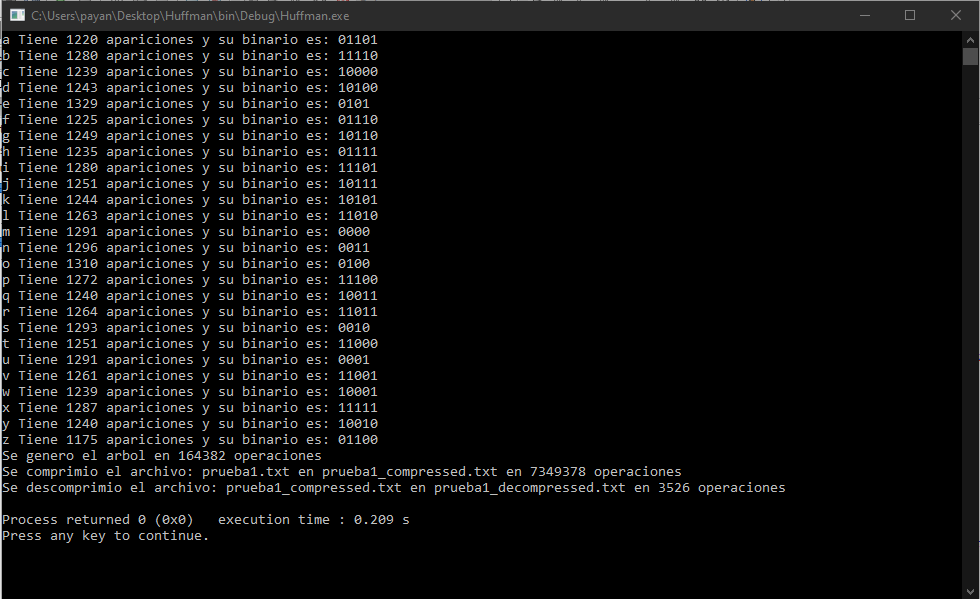
\includegraphics[width=400px,height=300px]{captura12}
		\caption{Ejecucion del programa}
	\end{figure}
	\begin{figure}[H]
		\centering
		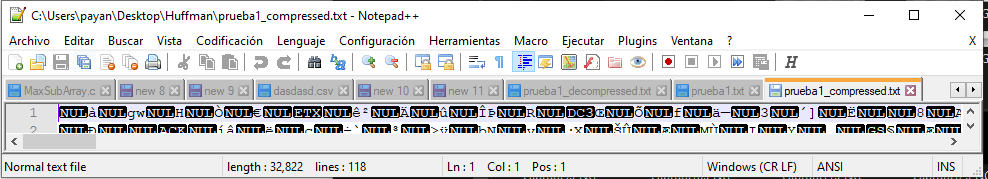
\includegraphics[width=400px,height=150px]{captura13}
		\caption{Archivo de salida}
	\end{figure}
	\begin{figure}[H]
		\centering
		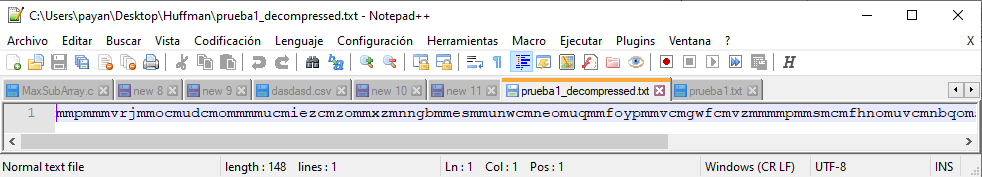
\includegraphics[width=400px,height=150px]{captura14}
		\caption{Archivo descomprimido}
	\end{figure}
	\begin{figure}[H]
		\centering
		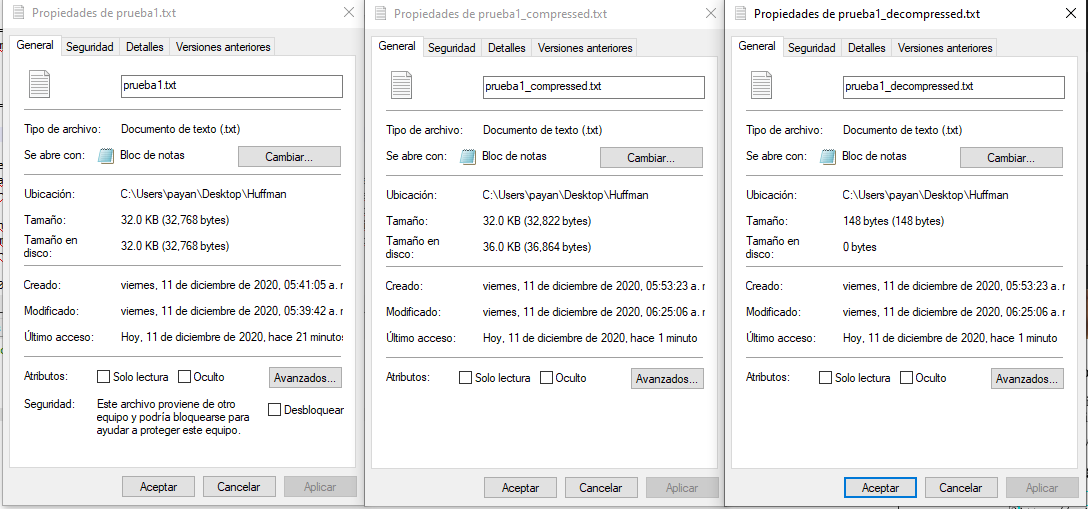
\includegraphics[width=400px,height=150px]{captura15}
		\caption{peso de los 3 archivos}
	\end{figure}
	\textbf{Segundo archivo}
	\begin{figure}[H]
		\centering
		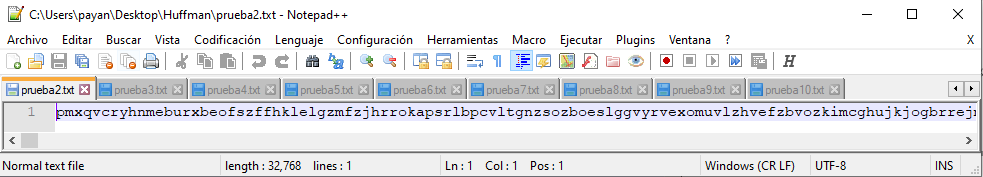
\includegraphics[width=400px,height=150px]{captura16}
		\caption{Archivo de entrada}
	\end{figure}
	\begin{figure}[H]
		\centering
		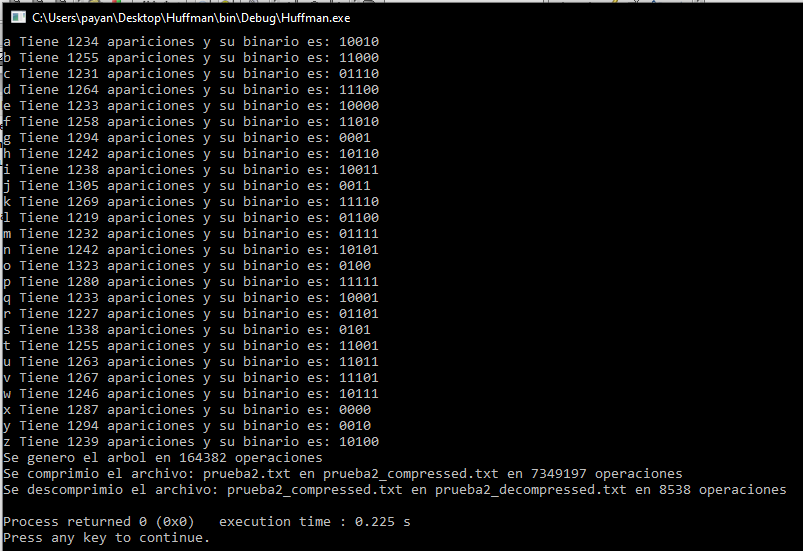
\includegraphics[width=400px,height=300px]{captura17}
		\caption{Ejecucion del programa}
	\end{figure}
	\begin{figure}[H]
		\centering
		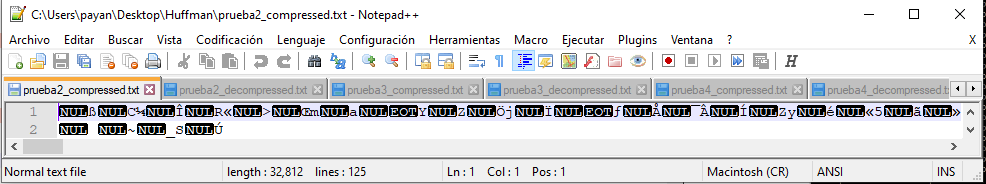
\includegraphics[width=400px,height=150px]{captura18}
		\caption{Archivo de salida}
	\end{figure}
	\begin{figure}[H]
		\centering
		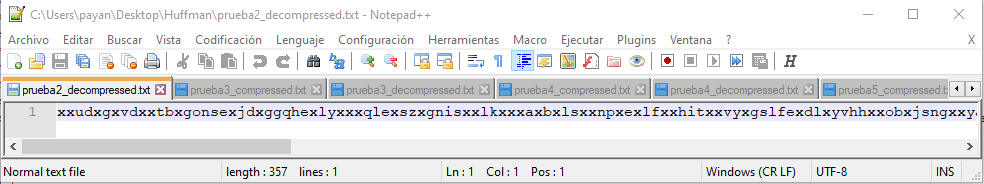
\includegraphics[width=400px,height=150px]{captura19}
		\caption{Archivo descomprimido}
	\end{figure}
	\begin{figure}[H]
		\centering
		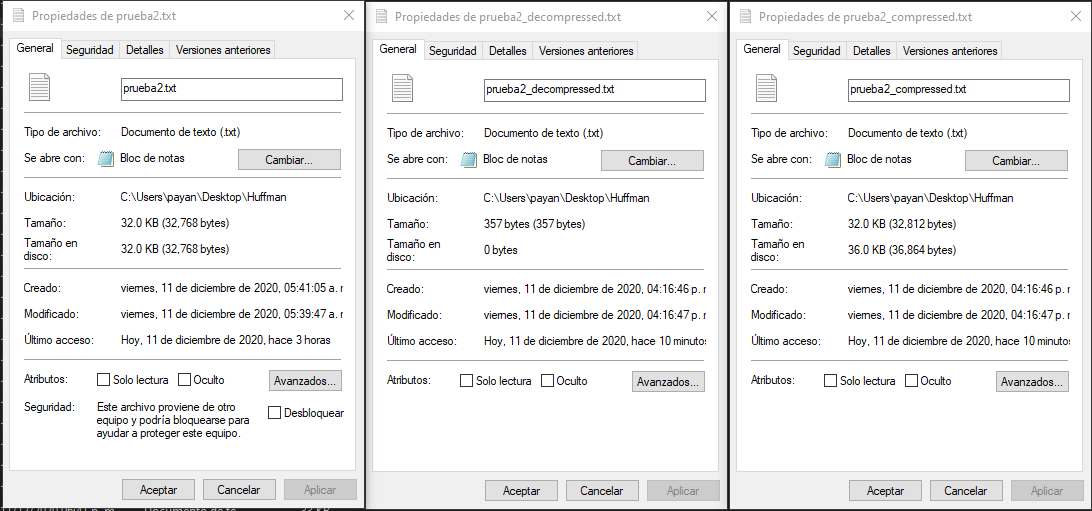
\includegraphics[width=400px,height=150px]{captura20}
		\caption{peso de los 3 archivos}
	\end{figure}
	\textbf{Tercer archivo}
	\begin{figure}[H]
		\centering
		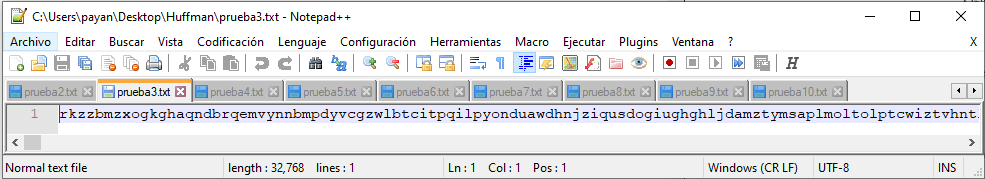
\includegraphics[width=400px,height=150px]{captura21}
		\caption{Archivo de entrada}
	\end{figure}
	\begin{figure}[H]
		\centering
		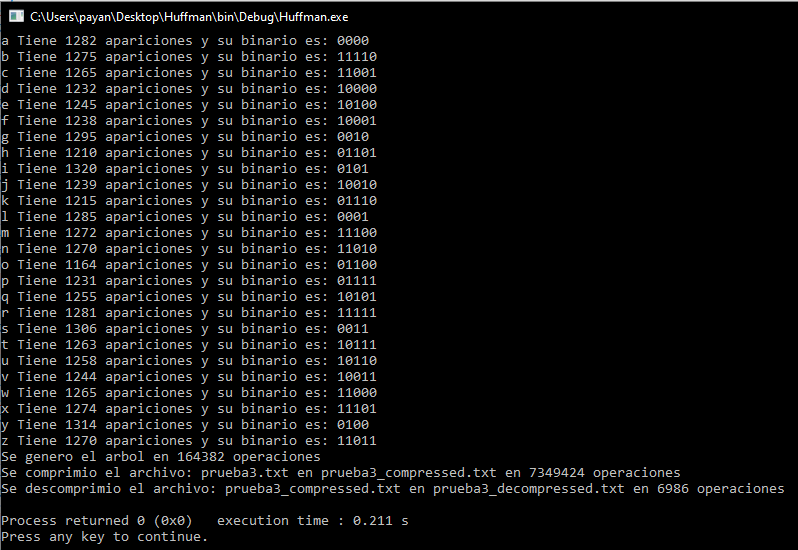
\includegraphics[width=400px,height=300px]{captura22}
		\caption{Ejecucion del programa}
	\end{figure}
	\begin{figure}[H]
		\centering
		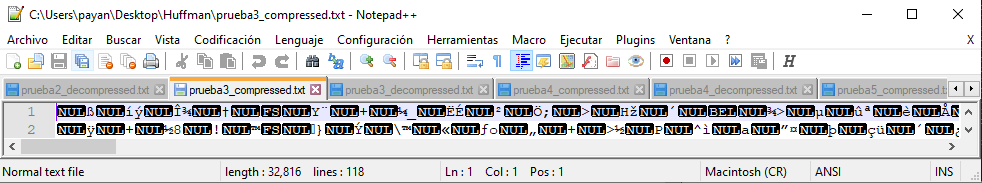
\includegraphics[width=400px,height=150px]{captura23}
		\caption{Archivo de salida}
	\end{figure}
	\begin{figure}[H]
		\centering
		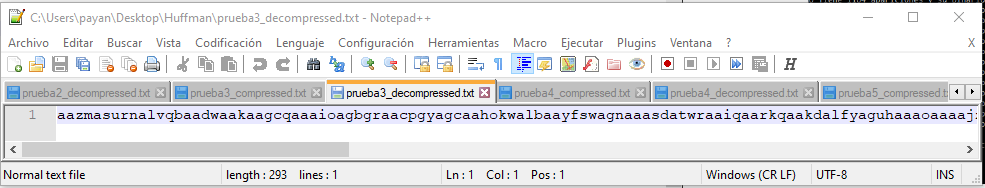
\includegraphics[width=400px,height=150px]{captura24}
		\caption{Archivo descomprimido}
	\end{figure}
	\begin{figure}[H]
		\centering
		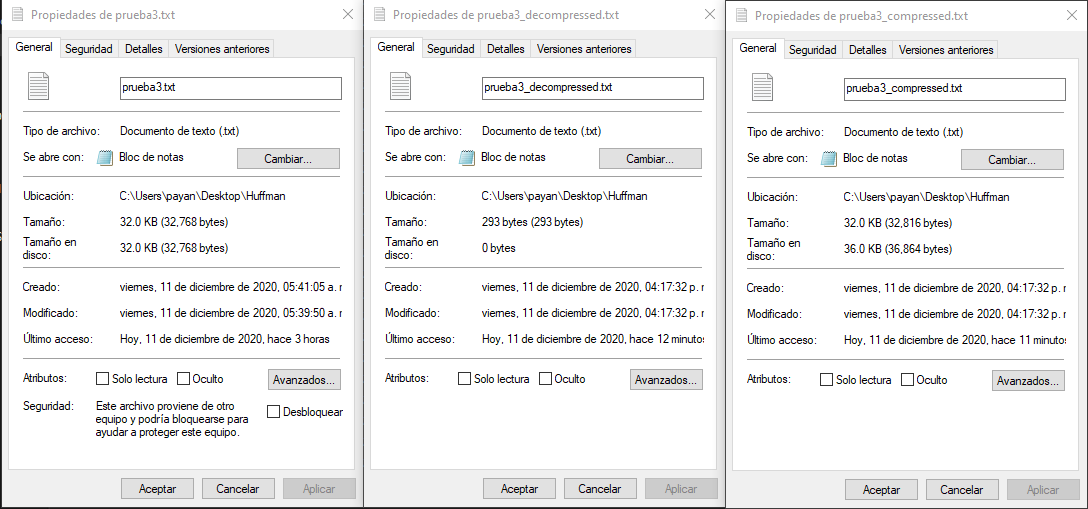
\includegraphics[width=400px,height=150px]{captura25}
		\caption{peso de los 3 archivos}
	\end{figure}
	\textbf{Cuarto archivo}
	\begin{figure}[H]
		\centering
		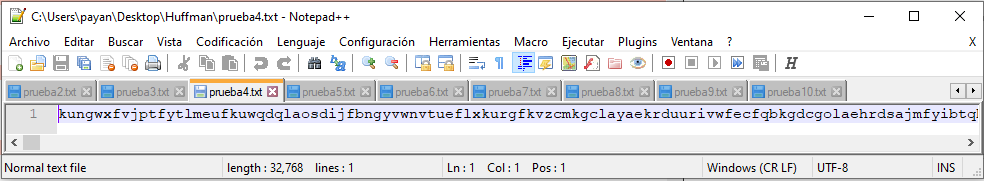
\includegraphics[width=400px,height=150px]{captura26}
		\caption{Archivo de entrada}
	\end{figure}
	\begin{figure}[H]
		\centering
		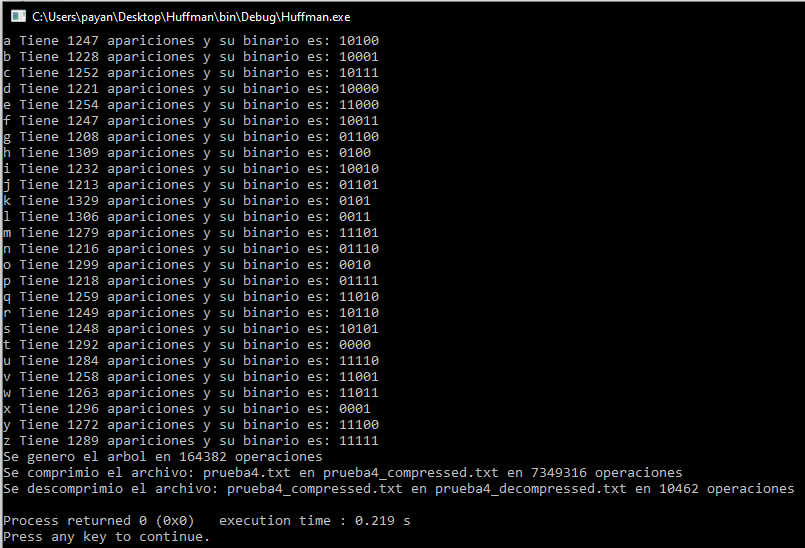
\includegraphics[width=400px,height=300px]{captura27}
		\caption{Ejecucion del programa}
	\end{figure}
	\begin{figure}[H]
		\centering
		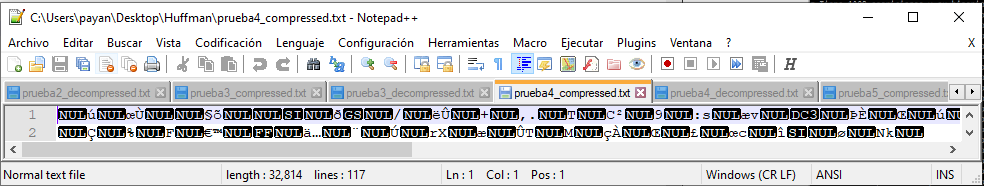
\includegraphics[width=400px,height=150px]{captura28}
		\caption{Archivo de salida}
	\end{figure}
	\begin{figure}[H]
		\centering
		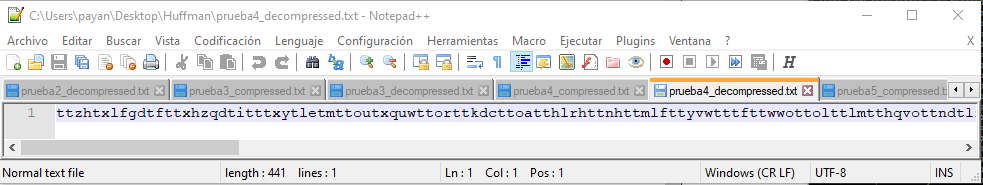
\includegraphics[width=400px,height=150px]{captura29}
		\caption{Archivo descomprimido}
	\end{figure}
	\begin{figure}[H]
		\centering
		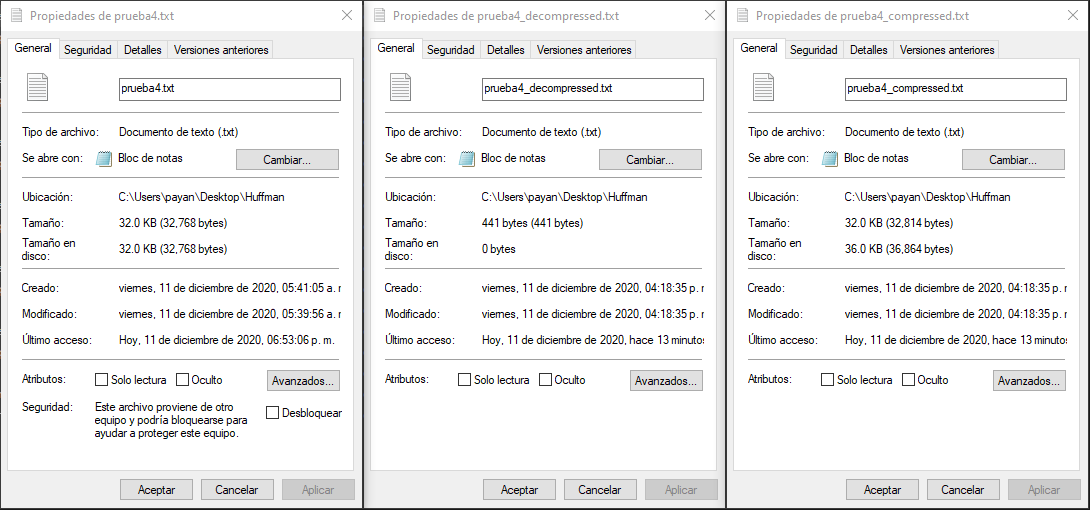
\includegraphics[width=400px,height=150px]{captura30}
		\caption{peso de los 3 archivos}
	\end{figure}
	\textbf{Quinto archivo}
	\begin{figure}[H]
		\centering
		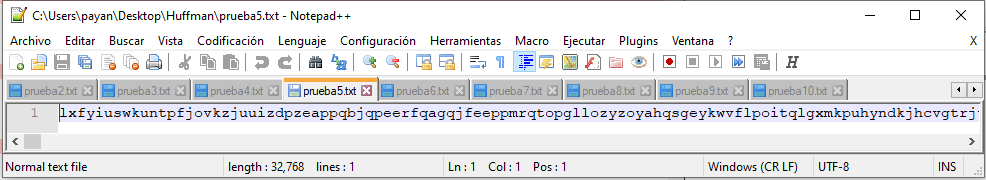
\includegraphics[width=400px,height=150px]{captura31}
		\caption{Archivo de entrada}
	\end{figure}
	\begin{figure}[H]
		\centering
		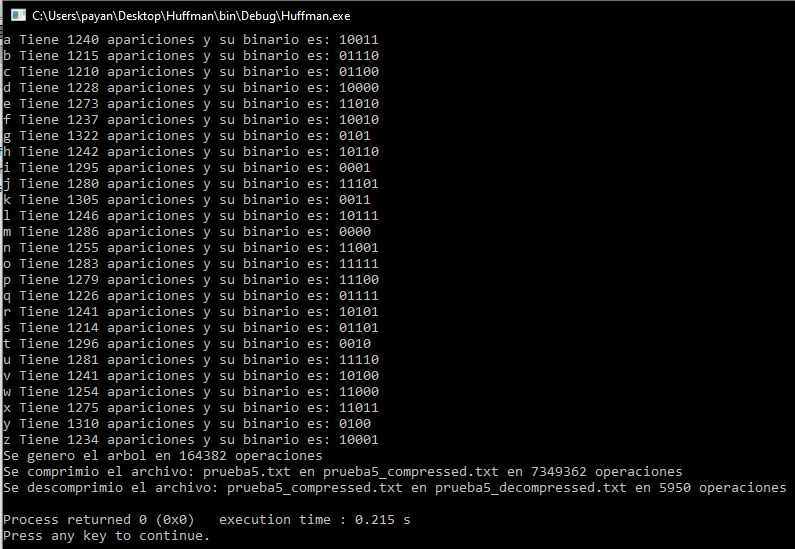
\includegraphics[width=400px,height=300px]{captura32}
		\caption{Ejecucion del programa}
	\end{figure}
	\begin{figure}[H]
		\centering
		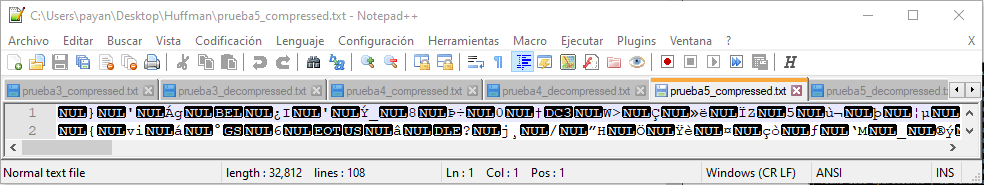
\includegraphics[width=400px,height=150px]{captura33}
		\caption{Archivo de salida}
	\end{figure}
	\begin{figure}[H]
		\centering
		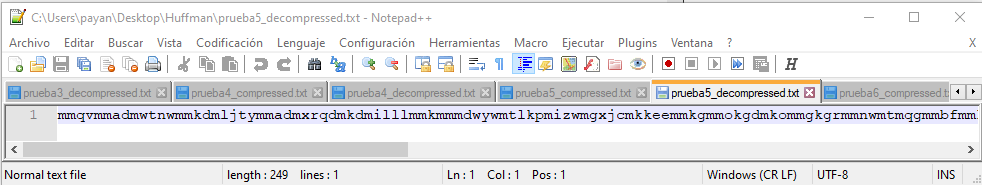
\includegraphics[width=400px,height=150px]{captura34}
		\caption{Archivo descomprimido}
	\end{figure}
	\begin{figure}[H]
		\centering
		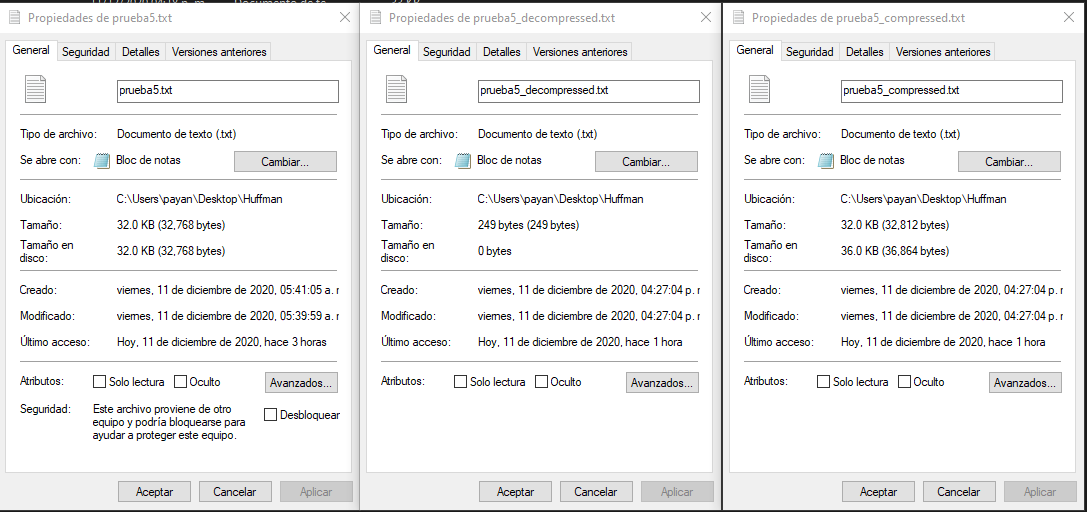
\includegraphics[width=400px,height=150px]{captura35}
		\caption{peso de los 3 archivos}
	\end{figure}
	\textbf{Sexto archivo}
	\begin{figure}[H]
		\centering
		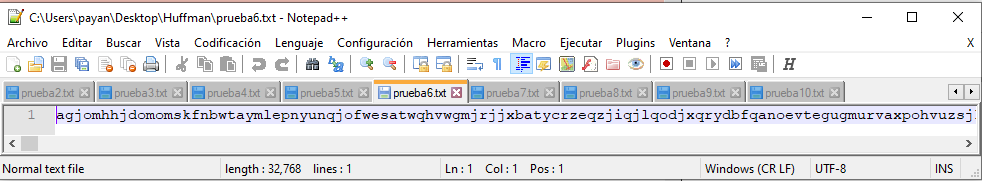
\includegraphics[width=400px,height=150px]{captura36}
		\caption{Archivo de entrada}
	\end{figure}
	\begin{figure}[H]
		\centering
		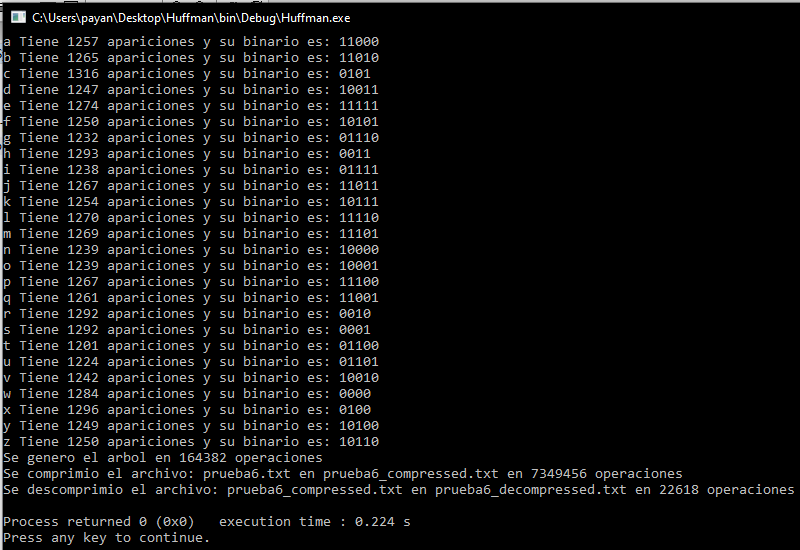
\includegraphics[width=400px,height=300px]{captura37}
		\caption{Ejecucion del programa}
	\end{figure}
	\begin{figure}[H]
		\centering
		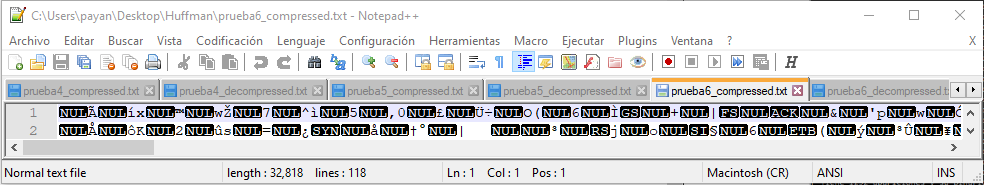
\includegraphics[width=400px,height=150px]{captura38}
		\caption{Archivo de salida}
	\end{figure}
	\begin{figure}[H]
		\centering
		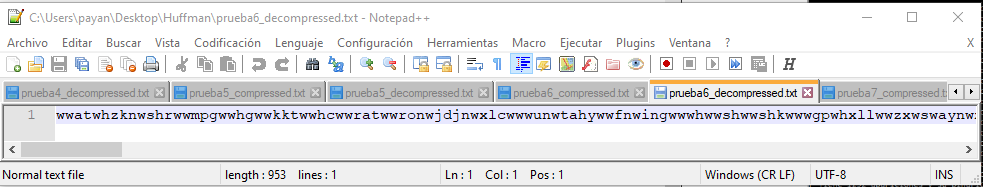
\includegraphics[width=400px,height=150px]{captura39}
		\caption{Archivo descomprimido}
	\end{figure}
	\begin{figure}[H]
		\centering
		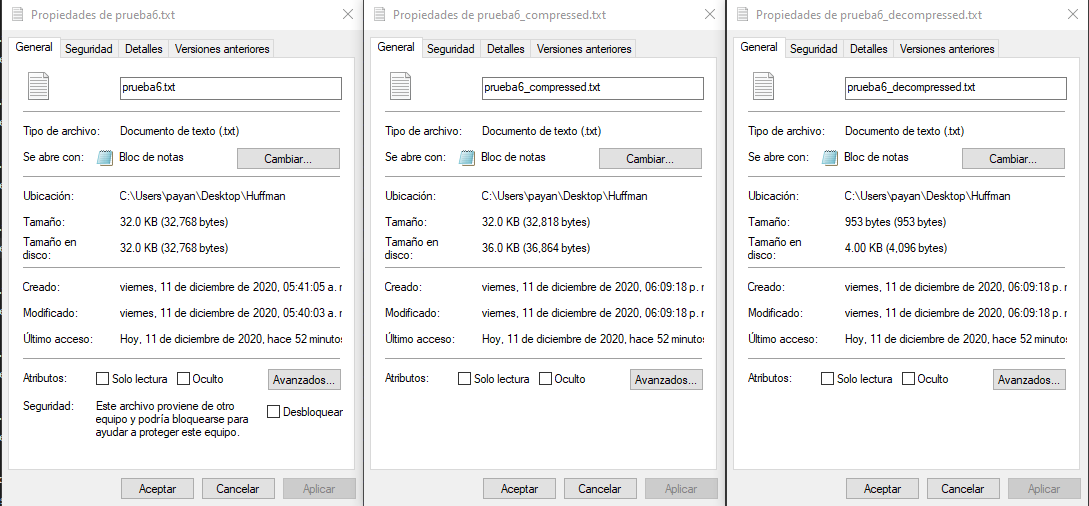
\includegraphics[width=400px,height=150px]{captura40}
		\caption{peso de los 3 archivos}
	\end{figure}
	\textbf{Septimo archivo}
	\begin{figure}[H]
		\centering
		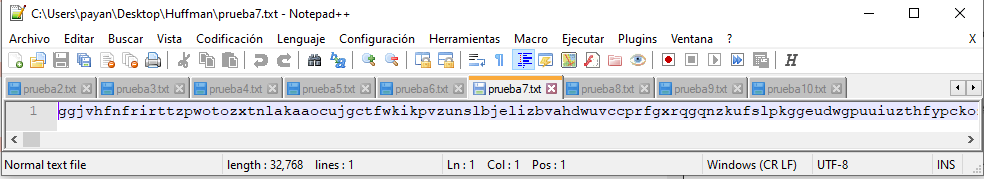
\includegraphics[width=400px,height=150px]{captura41}
		\caption{Archivo de entrada}
	\end{figure}
	\begin{figure}[H]
		\centering
		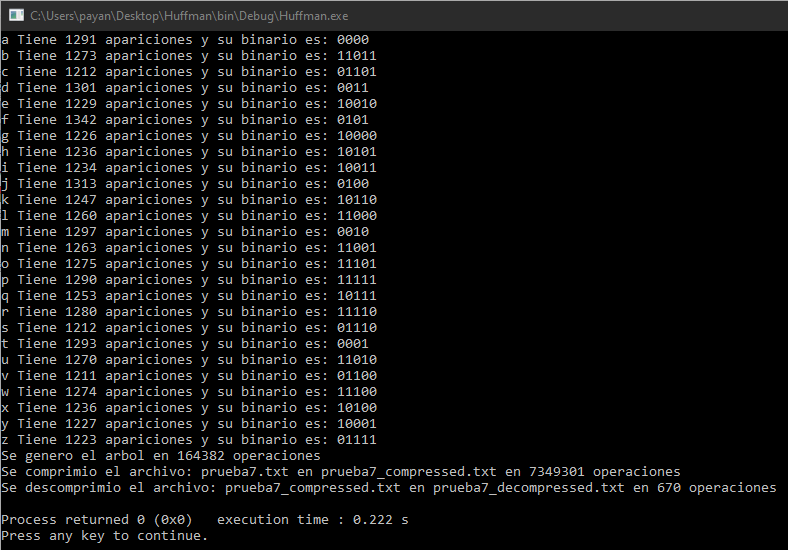
\includegraphics[width=400px,height=300px]{captura42}
		\caption{Ejecucion del programa}
	\end{figure}
	\begin{figure}[H]
		\centering
		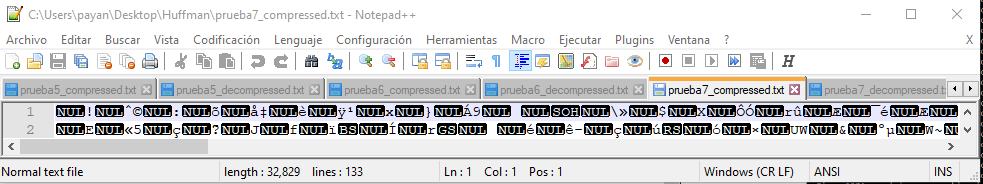
\includegraphics[width=400px,height=150px]{captura43}
		\caption{Archivo de salida}
	\end{figure}
	\begin{figure}[H]
		\centering
		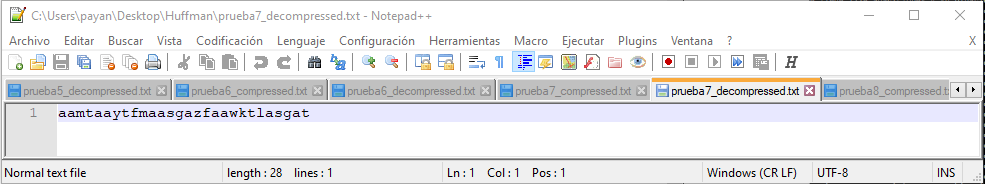
\includegraphics[width=400px,height=150px]{captura44}
		\caption{Archivo descomprimido}
	\end{figure}
	\begin{figure}[H]
		\centering
		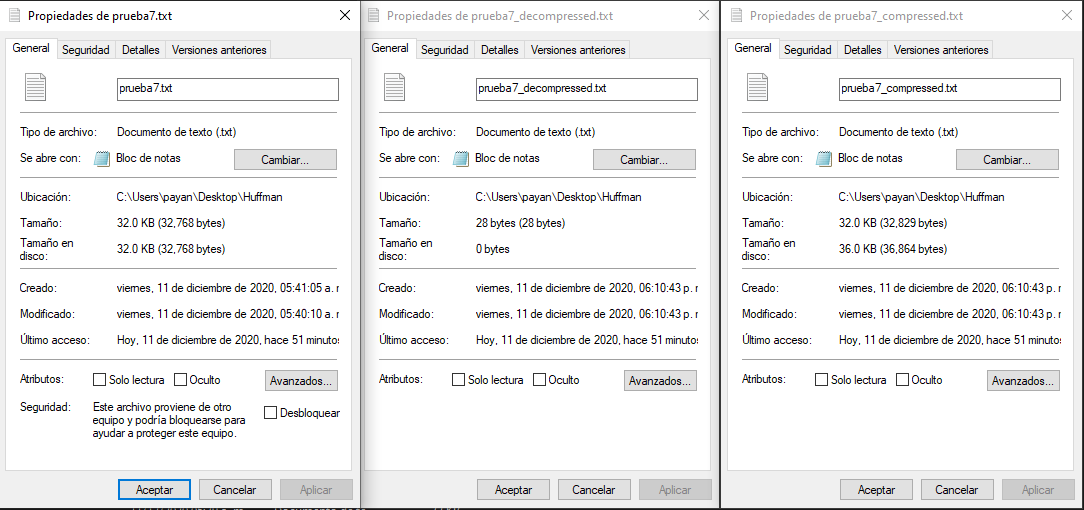
\includegraphics[width=400px,height=150px]{captura45}
		\caption{peso de los 3 archivos}
	\end{figure}
	\textbf{Octavo archivo}
	\begin{figure}[H]
		\centering
		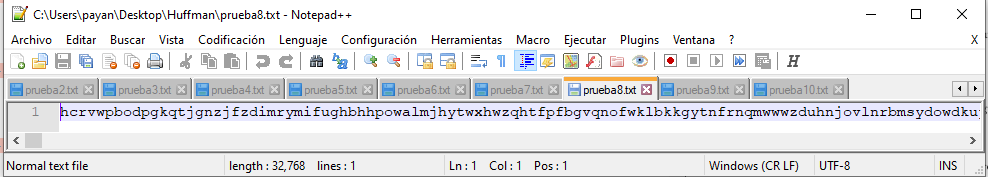
\includegraphics[width=400px,height=150px]{captura46}
		\caption{Archivo de entrada}
	\end{figure}
	\begin{figure}[H]
		\centering
		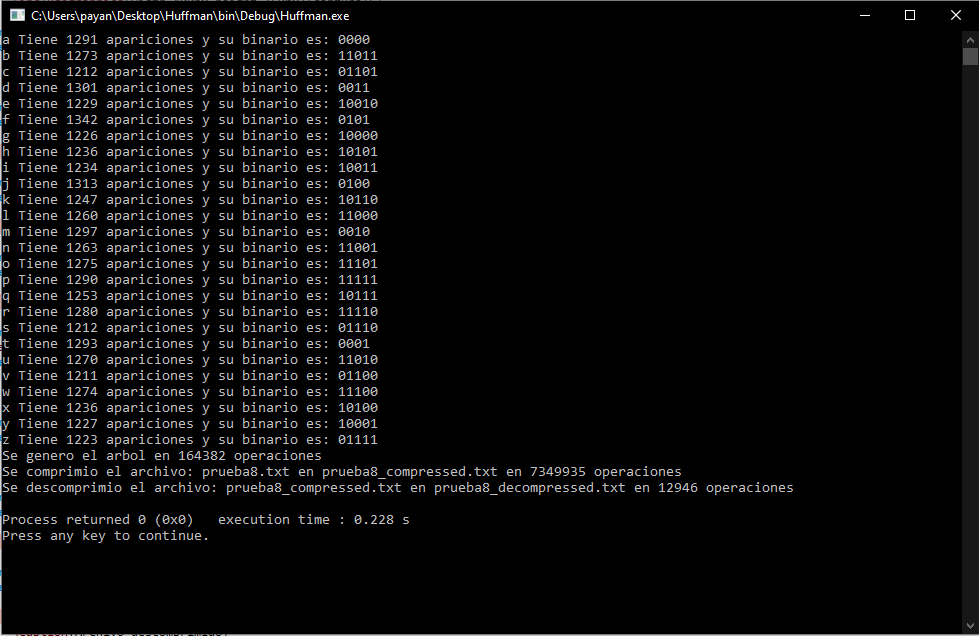
\includegraphics[width=400px,height=300px]{captura47}
		\caption{Ejecucion del programa}
	\end{figure}
	\begin{figure}[H]
		\centering
		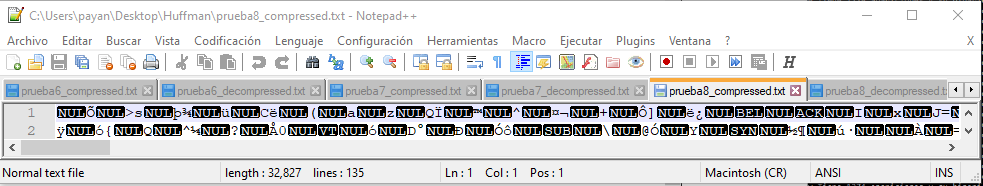
\includegraphics[width=400px,height=150px]{captura48}
		\caption{Archivo de salida}
	\end{figure}
	\begin{figure}[H]
		\centering
		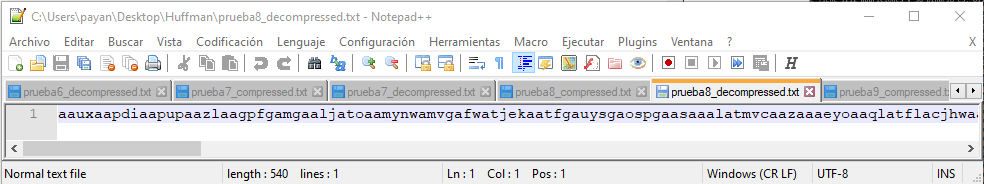
\includegraphics[width=400px,height=150px]{captura49}
		\caption{Archivo descomprimido}
	\end{figure}
	\begin{figure}[H]
		\centering
		\includegraphics[width=400px,height=150px]{captura50}
		\caption{peso de los 3 archivos}
	\end{figure}
	\textbf{Noveno archivo}
	\begin{figure}[H]
		\centering
		\includegraphics[width=400px,height=150px]{captura51}
		\caption{Archivo de entrada}
	\end{figure}
	\begin{figure}[H]
		\centering
		\includegraphics[width=400px,height=300px]{captura52}
		\caption{Ejecucion del programa}
	\end{figure}
	\begin{figure}[H]
		\centering
		\includegraphics[width=400px,height=150px]{captura53}
		\caption{Archivo de salida}
	\end{figure}
	\begin{figure}[H]
		\centering
		\includegraphics[width=400px,height=150px]{captura54}
		\caption{Archivo descomprimido}
	\end{figure}
	\begin{figure}[H]
		\centering
		\includegraphics[width=400px,height=150px]{captura55}
		\caption{peso de los 3 archivos}
	\end{figure}
	\textbf{Decimo archivo}
	\begin{figure}[H]
		\centering
		\includegraphics[width=400px,height=150px]{captura56}
		\caption{Archivo de entrada}
	\end{figure}
	\begin{figure}[H]
		\centering
		\includegraphics[width=400px,height=300px]{captura57}
		\caption{Ejecucion del programa}
	\end{figure}
	\begin{figure}[H]
		\centering
		\includegraphics[width=400px,height=150px]{captura58}
		\caption{Archivo de salida}
	\end{figure}
	\begin{figure}[H]
		\centering
		\includegraphics[width=400px,height=150px]{captura59}
		\caption{Archivo descomprimido}
	\end{figure}
	\begin{figure}[H]
		\centering
		\includegraphics[width=400px,height=150px]{captura60}
		\caption{peso de los 3 archivos}
	\end{figure}
	Finalmente para concluir este algorimo, se realizo una modificacion al codigo para generar una cadena aleatoria de longitud "$n$", con (1$\leq n\leq 10000$), posteriormente a esta se le genero el arbol, se comprimio y descomprimio, para poder obtener la grafica de complejidad de los algorimos de compresion y descompresion de Huffman.
	\begin{figure}[H]
		\centering
		\includegraphics[width=400px,height=300px]{grafica1}
		\caption{N contra operaciones de la generacion del arbol de Huffman}
	\end{figure}
	\begin{figure}[H]
		\centering
		\includegraphics[width=400px,height=300px]{grafica2}
		\caption{N contra operaciones de la codificacion de la cadena}
	\end{figure}
	\begin{figure}[H]
		\centering
		\includegraphics[width=400px,height=300px]{grafica3}
		\caption{N contra operaciones de la decodificacion de la cadena}
	\end{figure}
	\begin{figure}[H]
		\centering
		\includegraphics[width=400px,height=300px]{grafica4}
		\caption{N contra operaciones de la suma de la generacion del arbol de Huffman y compresion de la cadena}
	\end{figure}
	\begin{figure}[H]
		\centering
		\includegraphics[width=400px,height=300px]{grafica5}
		\caption{N contra operaciones de la suma de la generacion del arbol de Huffman y descompresion de la cadena}
	\end{figure}
	\begin{figure}[H]
		\centering
		\includegraphics[width=400px,height=300px]{grafica6}
		\caption{N contra operaciones de la suma de la generacion del arbol de Huffman, compresion y descompresion de la cadena}
	\end{figure}
	\begin{figure}[H]
		\centering
		\includegraphics[width=400px,height=300px]{grafica7}
		\caption{N contra operaciones comparando la generacion del arbol de Huffman y la compresion de datos}
	\end{figure}
	\begin{figure}[H]
		\centering
		\includegraphics[width=400px,height=300px]{grafica8}
		\caption{N contra operaciones comparando la generacion del arbol de Huffman y la descompresion de datos}
	\end{figure}
	\begin{figure}[H]
		\centering
		\includegraphics[width=400px,height=300px]{grafica9}
		\caption{N contra operaciones comparando la compresion y la descompresion de datos}
	\end{figure}
	\begin{figure}[H]
		\centering
		\includegraphics[width=400px,height=300px]{grafica7}
		\caption{N contra operaciones comparando la generacion del arbol de Huffman, la compresion de datos y la descompresion de los datos}
	\end{figure}
	\section{Conclusiones}			
	\subsection{Payán Téllez René}
	Esta practica se me hizo particulamente interesante porque los algoritmos que se trataron, no fueron tan directos de implementar en un lenguaje de programación, sin mencionar que algunas graficas tuvieron muy pocos valores, debido a lo complicado que era generar mas, porque computacionalmente su complejidad es inmensa. De hecho tuve que cambiar algunas variables de int a long long int en el espacio de los contadores para que siguiera funcionando el contador sin desbordarse. Tambien vi lo interesante de un algoritmo como MostrarPerfectos que tiene una complejidad no polinomial, ya que aunque lo puedo programar tardaria horas en encontrar mas alla del perfecto 5 (de por si toma mas de 5 minutos hallar el perfecto 4) sin mencionar que le tomaria dias encontrar otros números. Tambien cuando estaba demostrando la complejidad del algoritmo recursivo de la secuencia de fibonacci, algunos nucleos del CPU de mi computadora se dispararon, lo cual fue una señal de lo complicado y tardado que se podia volver en N muy grandes.\\
	\includegraphics[height=120px,width=120px]{Rene}
	\section{Anexo}			
	\subsection{Investigar el algoritmo de Karatsuba que permite obtener la multiplicación de enteros muy grandes}
	\subsection{Resolver los siguientes problemas}
	\section{Bibliografia}
		{[}1{]}\url{http://www.lcc.uma.es/~av/Libro/CAP3.pdf}\\
		{[}2{]}\url{https://medium.com/@joseguillermo_/qu\%C3\%A9-es-la-complejidad-algor\%C3\%ADtmica-y-con-qu\%C3\%A9-se-come-2638e7fd9e8c}\\
		{[}3{]}\url{https://www.tamps.cinvestav.mx/~ertello/algorithms/sesion15.pdf	}\\		
		{[}4{]}\url{http://elvex.ugr.es/decsai/algorithms/slides/4\%20greedy.pdf}\\		
		{[}5{]}\url{https://riptutorial.com/es/algorithm/example/23995/codificacion-huffman}\\		
	\end{document}